\documentclass[12pt]{article}

\usepackage[margin=1in]{geometry}
\usepackage{xcolor, color, soul}
\usepackage{amssymb}
\usepackage{enumitem}
\usepackage{booktabs}
\usepackage{amsmath}
\usepackage{array}
\usepackage{tabularx}
\usepackage{graphicx}
\usepackage{wrapfig}
\usepackage{blindtext}

\graphicspath{ {./images/} }
\sethlcolor{yellow}

\newcommand{\class}{Integral Calculus for Computer Science Students}
\newcommand{\datewritten}{Term 1, Fall '23}
\newcommand{\instructor}{Course Instructor: Noel T. Fortun}
\newcommand{\notes}{A.L. Maagma}
\newcommand{\follow}{\bigskip\noindent}
\newcommand{\spaces}{\quad\quad\quad}
\newcommand{\spacee}{\quad}
\newcommand{\point}{\,\cdot\,}

\newcommand{\mins}{-}
\newcommand{\block}[1]{\[{#1}\]}
\newcommand{\inline}[1]{\({#1}\)}
\newcommand{\proving}[1]{\begin{align*}{#1}\end{align*}}
\newcommand{\numbers}[1]{\begin{enumerate}[label*=\arabic*.]{#1}\end{enumerate}}
\newcommand{\enclose}[1]{\fbox{\parbox{\dimexpr\linewidth-2\fboxsep-2\fboxrule}{{#1}}}}

\newenvironment{conditions}
{\par\vspace{\abovedisplayskip}\noindent\begin{tabular}{>{$}l<{$} @{${}={}$} l}}
{\end{tabular}\par\vspace*{\belowdisplayskip}}

% ---------------- Start Document ----------------

\begin{document}
\pagestyle{plain}
\thispagestyle{empty}

% -------------------- Header --------------------

\noindent
\begin{tabular*}{\textwidth}{l @{\extracolsep{\fill}} r @{\extracolsep{6pt}} l}
    \textbf{\class} && \textbf{Date: \datewritten} \\
    \textbf{\instructor} && \textbf{Notes: \notes} \\
\end{tabular*}\\
\rule[2ex]{\textwidth}{2pt}

% ------------- Topic: Differentials -------------

\section{The Differentials}

    \enclose{
        \textbf{DEFINITION.}
        These provide us with a way of \hl{estimating the amount a function changes as a result of a small change in input values}.
        The equation \block{\triangle{y} \approx{} dy} can and will only be considered if \inline{\triangle{x}} is ``close enough''.
        The approximation of the equation becomes better as \inline{\triangle{x}} becomes smaller.
        
        \follow\textbf{NOTE.}
        We equate \inline{\triangle{x} = dx}.
    }

    \subsection{The Differential of the Independent Variable}

        \enclose{
            \textbf{DEFINITION.}
            If the function \textit{f} is definited by the equation \inline{y = f (x)}, then the \hl{differential of y}, denoted by \textit{dy}, is given by \block{dy = f' (x) \, dx \longrightarrow{} f' (x) = \frac{dy}{dx}} where \textit{x} is any number in the domain of \textit{f'} and \inline{\triangle{x}} is an arbitrary increment of \textit{x}.
        }

        \follow\textbf{EXAMPLE 1.1.1.}
        Find \textit{dy} for \inline{y = (x^3 + 5x \mins{} 1)^{2023}}.
        \block{f' (x) = 2023 (x^3 + 5x \mins{} 1)^{2022} (3x^2 + 5)}
        \block{\therefore{} dy = 2023(x^3 + 5x \mins{} 1) (3x^2 + 5x) \, dx}

        \follow\textbf{EXAMPLE 1.1.2.}
        Find the differential \textit{dy} of the function \inline{y = 4x^2 + x + 3}.
        \block{(8x + 1) \, dx}

        \follow\textbf{EXAMPLE 1.1.3.}
        Find the differential \textit{dy} of the function \inline{y = \cos(x)}.
        \block{dy = \mins{} \sin(x) \, dx}

        \newpage\follow\textbf{NOTE.}
        The following figures represent the corresponding derivatives of trigonometric identities or functions.
        
        \follow\begin{center}\begin{tabular}{ccc}
            \toprule \inline{f (x)} && \inline{f' (x)} \\
            \midrule \inline{\sin(x)} && \inline{\cos(x)} \\ 
            \midrule \inline{\cos(x)} && \inline{\mins{} \sin(x)} \\
            \midrule \inline{\tan(x)} && \inline{\sec^2 (x)} \\
            \midrule \inline{\cot(x)} && \inline{\mins{} \csc^2 (x)} \\
            \midrule \inline{\sec(x)} && \inline{\sec(x) \tan(x)} \\
            \midrule \inline{\csc(x)} && \inline{\mins{} \csc(x) \cot(x)} \\
        \bottomrule\end{tabular}\end{center}

        \follow\textbf{EXAMPLE 1.1.4.}
        Compare the values of \inline{\triangle{y}} and \textit{dy} if \inline{y = f (x) = x^3 + x^2 \mins{} 2x + 1} and \textit{x} changes (a) from 2 to 2.05 and (b) from 2 to 2.01.
        
        \begin{align*}
            x &= 2                  & \triangle{y} &= f(x + \triangle{x}) - f(x)& dy &= f'(x) \, dx \\
            x + \triangle{x} &= 2.05& &= f(2.05) - f(2)                         & &= (3x^2 + 2x \mins 2) \, dx \\
            \triangle{x} &= 0.05    & &= 0.7176                                 & &= (3{(2)}^2 + 2(2) \mins 2)(0.05) \\
            dx &= 0.05              &&                                          & &= 0.7
        \end{align*}

        \follow\textbf{NOTE.}
        The final equation utilized our solution at \inline{x = 2}, \inline{\triangle{x} = dx = 0.05}.
        Observe the approximation of \inline{\triangle{y} \approx{} dy} becomes better as \inline{\triangle{x}} becomes smaller.

    \subsection{Error Propagation}

        \enclose{
            \textbf{DEFINITION.}
            In practice, differentials can be used in the estimation of errors propagated by physical measuring devices.
            If the measure value of \textit{x} is used to compute another value \inline{f (x)}, then the difference between \inline{f (x + \triangle{x})} and \textit{f (x)} is the propagated error.
            
            \block{f (x + \triangle{x}) \mins{} f (x) = \triangle{y} \approx{} dy} where:
            
            \begin{conditions}
                x + \triangle{x} & Exact Value \\
                \triangle{x} & Measurement Error \\
                f (x) & Measured Value \\
                \triangle{y} & Propagated Error
            \end{conditions}

            \textbf{NOTE.}
            How do you know if the propagated error is large or small?
            The answer is best given in \textit{relative} terms by comparing \textit{dA} and \textit{A}.
            The ratio is called the \hl{relative error} and further be expressed as \hl{percentage error}.
        }

        \follow\textbf{EXAMPLE 1.2.1}
        A radius of a sphere is to be 3 cm with a possible error of 0.02 cm. (1) Use differentials to approximate the error in calculating the volume. (2) What is the relative error and percentage error?

        \begin{align*}
            && V &= \frac{4}{3} \pi r^3 \\
            dV &= V' \, dr              &&& \frac{dV}{V} &= \frac{\pm 2.2619}{36 \pi} \\
            &= 4 \pi r^2 \, dr          &&& (2.1) &= \pm 0.02 \\
            &= 4 \pi {(3)}^2 (\pm 0.02) &&& (2.2) &= \pm 2\% \\
            (1) &= \pm 2.2619 \, cm^3
        \end{align*}

        \follow\textbf{SUMMARY.}
        The essence of differentials provide us with a way of estimating the amount a function changes as a result of a small change in input values.

        \follow\textbf{REMARK.}
        Although the application of differentials to approximate function values is not very important in the age of technology, differentials are important as a \hl{convinient notational device} for the computation of antiderivatives.

\section{Antidifferentiation: Indefinite Integration}

    \textbf{EXAMPLE 2.0.1}
    In order to find a function \textit{F} whose derivative is \inline{F' (x) = 3x^2}, we use our knowledge of derivatives to conclude the following: \block{F (x) = x^3 \; \textrm{since} \; \frac{d}{dx}[x^3] = 3x^2}
    The function \textit{F} is considered an antiderivative of \textit{f}.

    \follow\enclose{
        \textbf{DEFINITION.}
        A function \textit{F} is \hl{an antiderivative} of \textit{f} of an interval \textit{I} when \block{F' (x) = f (x)} for all \textit{x} in \textit{I}.
        As for the previous example, \inline{F (x) = x^3} is an antiderivative of \inline{f (x) = 3x^2}.

        \follow\textbf{NOTE.}
        An antiderivative of \textit{f} is not unique because of the infinite possible values for the constant \textit{C}.
    }

    \subsection{General Antiderivative of a Function}

        \enclose{
            \textbf{DEFINITION.}
            If \textit{F} \hl{is an antiderivative of \textit{f}} on an interval \textit{I}, then G \hl{is an antiderivative of \textit{f}} on the interval \textit{I} if and only if \textit{G} is of the form \block{G (x) = F (x) + C} for all \textit{x} in \textit{I}, where \textit{C} is a constant.
        }

        \follow\enclose{
            \textbf{DEFINITION.}
            The operation of finding the antiderivatves of a function is called \hl{antidifferentiation}, or indefinite integration, and is denoted by an integral sign \inline{\int{}}. 
            Additionally, the equation below states that when we antidifferentiate the differential of a function, we obtain the function plus an arbitrary constant. 
            \block{\int{} f (x) \, dx = F (x) + C}
            \begin{conditions}
                \int{} & Integration Symbol \\
                f (x) & Integrand \\
                dx & Differential of X \\
                F (x) & One Antiderivative \\
                C & Constant of Integration
            \end{conditions}
            
            \textbf{NOTE.}
            The expression \inline{\int{} f (x) \, dx} is read as ``the antiderivative of f with respect to x''. The differential \textit{dx} serves to identify \textit{x} as the variable of integration. The term \hl{indefinite integral} is a synonym for antiderivative.
        }

    \subsection{Basic Integration Rules}

        \bigskip\begin{center}\begin{tabular}{ccc}
            \toprule\ \textbf{Differentiation Formula} && \textbf{Integration Formula} \\
            \midrule\ \inline{\frac{d}{dx}[C] = 0} && \inline{\int{} 0 \, dx = C} \\
            \midrule\ \inline{\frac{d}{dx}[kx] = k} && \inline{\int{} k \, dx = kx + C} \\
            \midrule\ \inline{\frac{d}{dx}[kf (x)] = kf' (x)} && \inline{\int{} kf (x) \, dx = k \int{} f (x) \, dx} \\
            \midrule\ \inline{\frac{d}{dx}[f (x) \pm{} g (x)] = f' (x) \pm{} g ' (x)} && \inline{\int{} [f (x) \pm{} g (x)] \, dx = \int{} f (x) \, dx \pm{} \int{} g (x) \, dx} \\ 
            \midrule\ \inline{\frac{d}{dx}[x^n] = {nx}^{n \mins{} 1}} && \inline{\int{} x^n \, dx = \frac{x^{n + 1}}{n + 1} + C}, \inline{n \neq{} \mins{} 1} \\
            \midrule\ \inline{\frac{d}{dx}[\sin{x}] = \cos{x}} && \inline{\int{} \cos{x} \, dx = \sin{x} + C} \\
            \midrule\ \inline{\frac{d}{dx}[\cos{x}] = \mins{} \sin{x}} && \inline{\int{} \sin{x} \, dx = \mins{} \cos{x} + C} \\
            \midrule\ \inline{\frac{d}{dx}[\tan{x}] = \sec^2{x}} && \inline{\int{} sec^2{x} \, dx = \tan{x} + C} \\
            \midrule\ \inline{\frac{d}{dx}[\sec{x}] = \sec{x} \tan{x}} && \inline{\int{} \sec{x} \tan{x} \, dx = \sec{x} + C} \\
            \midrule\ \inline{\frac{d}{dx}[\cot{x}] = \mins{} \csc^2{x}} && \inline{\int{} \csc^2{x} \, dx = \mins{} \cot{x} + C} \\
            \midrule\ \inline{\frac{d}{dx}[\csc{x}] = \mins{} \csc{x} \cot{x}} && \inline{\int{} \csc{x} \cot{x} \, dx = \mins{} \csc{x} + C} \\
        \bottomrule\end{tabular}\end{center}

    \subsection{Power Rule of Integrals}

        \enclose{
            \textbf{DEFINITION.}
            As for the power rule of integrals, as long as \inline{n \neq{} 1},
            \block{\int{} x^n \, dx = \frac{x^{n + 1}}{n + 1} + C}
        }

        \follow\textbf{EXAMPLE 2.3.1.}
        Find the antiderivative of \inline{\int{} x^5 \, dx}.
        \proving{
            &= \frac{x^6}{6} + C
        }

        \follow\textbf{EXAMPLE 2.3.2.}
        Find the antiderivative of \inline{\int{} \sqrt{x} \, dx}.
        \proving{
            &= \int{} x^{1/2} \, dx \\
            &= \frac{x^{\frac{1}{2} + 1}}{\frac{1}{2} + 1} + C \\
            &= \frac{x^{\frac{3}{2}}}{\frac{3}{2}} + C \\
            &= \frac{2 x^{\frac{3}{2}}}{3} + C
        }

        \follow\textbf{EXAMPLE 2.3.3.}
        Find the antiderivative of \inline{\int{} 3x \, dx}.
        \proving{
            &= 3 \int{} x \, dx \\
            &= 3 \point{} \frac{x^2}{2} \\
            &= \frac{3x^2}{2} + C
        }

        \follow\textbf{EXAMPLE 2.3.4.}
        Find the antiderivative of \inline{\int{} \frac{1}{x^3} \, dx}.
        \proving{
            &= \mins{} \frac{1}{2x^2} + C
        }

        \follow\textbf{EXAMPLE 2.3.5.}
        Find the antiderivative of \inline{\int{} 2 \sin{x} \, dx}.
        \proving{
            &= 2 \int{} \sin{x} \, dx \\
            &= 2 \point{} \mins{} \cos{x} \\
            &= \mins{} 2 \cos{x} + C
        }

        \follow\textbf{EXAMPLE 2.3.6.}
        Find the antiderivative of \inline{\int{} (3x^4 \mins{} 5x^2 + x) \, dx}.
        \proving{
            &= 3 \int{} x^4 \, dx \mins{} 5 \int{} x^2 \, dx + \int{} x \, dx \\
            &= \frac{3x^5}{5} \mins{} \frac{5x^3}{3} + \frac{2x^2}{2} + C
        }

        \follow\textbf{EXAMPLE 2.3.7.}
        Find the antiderivative of \inline{\int{} \frac{x + 1}{\sqrt{x}} \, dx}.
        \proving{
            && &= \int{} \left(\frac{x}{\sqrt{x}} + \frac{1}{\sqrt{x}}\right) \, dx \\
            && &= \int{} \left(\sqrt{x} + \frac{1}{\sqrt{x}}\right) \, dx \\
            &= \int{} \sqrt{x} \, dx &&& &= \int{} \frac{1}{\sqrt{x}} \, dx \\
            &= \int{} x^{\frac{1}{2}} \, dx &&& &= \int{} x^{\mins{} \frac{1}{2}} \, dx \\
            &= \frac{2 \sqrt{x^3}}{3} &&& &= 2 \sqrt{x} \\
            && &= \frac{2 \sqrt{x^3}}{3} + 2 \sqrt{x} \\
            && &= \frac{2 \sqrt{x} (x + 3)}{3} + C
        }

        \follow\textbf{NOTE.}
        The following are reciprocal and pythagorean identities for trigonometric integrals.
        \proving{
            \cot{x} &= \frac{1}{\tan{x}} = \frac{\cos{x}}{\sin{x}} & \sin^2{x} &+ \cos^2{x} = 1 \\
            \csc{x} &= \frac{1}{\sin{x}} & \sec^2{x} &= 1 + \tan^2{x} \\
            \sec{x} &= \frac{1}{\cos{x}} & \csc^2{x} &= 1 + \cot^2{x}
        }
        

        \follow\textbf{EXAMPLE 2.3.8.}
        Find the antiderivative of \inline{\int{} \frac{\sin{x}}{\cos^2{x}} \, dx}.
        \proving{
            &= \int{} \frac{\sin{x}}{\cos{x}} \point{} \frac{1}{\cos{x}} \, dx \\
            &= \int{} \tan{x} \sec{x} \, dx \\
            &= \frac{1}{\cos{x}} + C \\
            &= \sec{x} + C
        }

        \follow\textbf{EXAMPLE 2.3.9.}
        Find the antiderivative of \inline{\int{} \sec{\theta} (\sec{\theta} + \tan{\theta}) \, d\theta{}}.
        \proving{
            &= \int{} (\sec^2{\theta} + \sec{\theta} \tan{\theta}) \, d \theta{} \\
            &= \int{} \sec^2{\theta} \, d\theta{} + \int{} \sec{\theta} \tan{\theta} \, d\theta{} \\
            &= \tan{\theta} + \sec{\theta} + C
        }

\section{Integration by Substitution}

    \enclose{
        \textbf{DEFINITION.}
        If \inline{u = g (x)} is a differentiable function whose range is an interval \textit{I} and \textit{f} is continuous on \textit{I}, then \block{\int{} f (g (x)) g' (x) \, dx = \int{} f (u) \, du}
    }

    \follow\textbf{EXAMPLE 3.0.1.}
    Find the antiderivative of \inline{\int{} (x^2 + 5) \, 2x \, dx}.
    \proving{
        &= \int{} (2x^3 + 10x) \, dx \\
        &= \frac{2x^4}{4} + \frac{10x^2}{2} + C \\
        &= \frac{x^4}{2} + 5x^2 + C
    }

    \follow\textbf{EXAMPLE 3.0.2.}
    Find the antiderivative of \inline{\int{} (x^2 + 5)^{100} \, 2x \, dx}.
    
    \begin{align*}
        u &= x^2 + 5 & &= \int{} u^{100} \, du \\
        du &= 2x + dx & &= \frac{u^{100}}{101} + C \\
        && &= \frac{{(x^2 + 5)}^{101}}{101} + C
    \end{align*}

    \subsection{Chain Rule for Antidifferentiation}
    
        \enclose{
            \textbf{DEFINITION.}
            If we consider F and \textit{f} such that \inline{F' = f} (\textit{F} is an antiderivative of \textit{f}) and supposing we have a composition \inline{F (g (x))}, then by chain rule for differentiation,
            \proving{
                \frac{d}{dx} [F (g (x))] &= F' (g (x)) \point{} g' (x) \\
                \int{} F' (g (x)) \point{} g' (x) \, dx &= F (g (x)) + C \\
                \int{} F' (g (x)) \point{} g' (x) \, dx &= \int{} F' (u) \, du \\
                \int{} f (g (x)) \point{} g' (x) \, dx &= \int{} f (u) \, du
            }
        }

        \follow\textbf{EXAMPLE 3.1.1.}
        Find the antiderivative of \inline{\int{} \sqrt{3x + 4} \, dx}.

        \begin{align*}
            f(x) &= \sqrt{x}        &&= \int{} \sqrt{3x + 4} \, dx                      & u &= 3x + 4 \\
            g(x) &= 3x + 4          &&= \frac{1}{3} \int{} {(3x + 4)}^{1/2} (3 \, dx)   & du &= 3 \, dx \\
            f(g(x)) &= f(3x + 4)    &&= \frac{1}{3} \int{} u^{1/2} \, du \\
            &= \sqrt{3x + 4}        &&= \frac{1}{3} \point{} \frac{u^{3/2}}{3/2} + C \\
            &                       &&= \frac{1}{3} \point{} \frac{2}{3} u^{3/2} + C \\
            &                       &&= \frac{2}{9} {(3x + 4)}^{3/2} + C
        \end{align*}

        \follow\textbf{EXAMPLE 3.1.2.}
        Find the antiderivative of \inline{\int{} \frac{4x^2}{{(1 \mins{} 8x^3)}^4} \, dx}.

        \begin{align*}
            &= \mins{} \frac{1}{6} \int{} {(1 \mins{} 8x^3)}^{\mins{} 4} (\mins{} 6 \point{} 4x^2 \, dx)    & u &= 1 \mins{} 8x^3 \\
            &= \mins{} \frac{1}{6} \int{} u^{\mins{} 4} \, du                                               & du &= \mins{} 24x^2 \, dx \\
            &= \mins{} \frac{1}{6} \point{} \frac{u^{\mins{} 3}}{\mins{} 3} + C \\
            &= \frac{1}{18} u^{\mins{} 3} + C \\
            &= \frac{1}{18} {(1 \mins{} 8x^3)}^{\mins{} 3} + C
        \end{align*}
        
        \newpage\follow\textbf{EXAMPLE 3.1.3.}
        Find the antiderivative of \inline{\int{} x^2 \sqrt{1 + x} \, dx}.

        \begin{align*}
            &= \int{} {(u \mins{} 1)}^2 u^{1/2} \, du                                                               & u &= 1 + x        & x &= u \mins{} 1 \\
            &= \int{} {(u^2 \mins{} 2u + 1)} u^{1/2} \, du                                                          & du &= dx          & x^2 &= {(u \mins{} 1)}^2 \\
            &= \int{} (u^{5/2} \mins{} 2u^{3/2} + u^{1/2}) \, du                                                    \\
            &= \frac{2}{7} u^{7/2} \mins{} \frac{4}{5} u^{5/2} + \frac{2}{3} u^{3/2} + C                            \\
            &= \frac{2}{7} {(1 + x)}^{7/2} \mins{} \frac{4}{5} {(1 + x)}^{5/2} + \frac{2}{3} {(1 + x)}^{3/2} + C
        \end{align*}

        \follow\textbf{EXAMPLE 3.1.4.}
        Find the antiderivative of \inline{\int{} \sin{x} \sqrt{1 \mins{} \cos{x}} \, dx}.

        \begin{align*}
            &= \int{} \sqrt{u} \, du    & u &= 1 \mins{} \cos{x} \\
            &= \int{} {(u)}^{1/2} \, du & du &= \sin{x} \, dx \\
            &= \frac{2}{3} \sqrt{u^3} \\
            &= \frac{2}{3} \sqrt{{(1 \mins{} \cos{x})}^3} + C
        \end{align*}

        \follow\textbf{EXAMPLE 3.1.5.}
        Find the antiderivative of \inline{\int{} (x + 1) \sqrt{(2x + x^2)} \, dx}.
        
        \begin{align*}
            &= \int{} \sqrt{u} (x + 1) \, dx                        & u &= 2x + x^2 \\
            &= \frac{1}{2} \int{} \sqrt{u} \, du                    & du &= 2x + 2 \\
            &= \frac{1}{2} \int{} {(u)}^{1/2} \, du \\
            &= \frac{1}{2} \point{} \frac{2}{3} {(u)}^{3/2} + C \\
            &= \frac{1}{3} {(x^2 + 2x)}^{3/2} + C
        \end{align*}

        \newpage\follow\textbf{EXAMPLE 3.1.6.}
        Find the antiderivative of \inline{\int{} \frac{x^2}{\sqrt[3]{1 + x^3}} \, dx}.

        \begin{align*}
            &= \int{} \frac{x^2}{\sqrt[3]{u}} \, dx                 & u &= 1 + x^3 \\
            &= \frac{1}{3} \int{} \frac{du}{\sqrt[3]{u}}            & du &= 3x^2 \, dx \\
            &= \frac{1}{3} \int{} {(u)}^{\mins 1/3} \, du \\
            &= \frac{1}{3} \point{} \frac{3}{2} {(u)}^{2/3} + C \\
            &= \frac{{(1 + x^3)}^{2/3}}{2} + C
        \end{align*}

        \follow\textbf{EXAMPLE 3.1.7.}
        Find the antiderivative of \inline{\int{} x \sqrt{x + 2} \, dx}.
        
        \begin{align*}
            &= \int{} (u \mins{} 2) {(u)}^{1/2} \, du       & u &= x + 2 \\
            &= \int{} (u^{3/2} \mins{} 2u^{1/2}) \, du      & du &= dx \\
            &= \frac{1}{2} \left(\frac{2}{5} u^{5/2} \mins{} \frac{4}{3} u^{3/2}\right) \\
            &= \frac{2}{5} u^{5/2} \mins{} \frac{4}{3} u^{3/2} + C \\
            &= \frac{2}{5} {(x + 2)}^{5/2} \mins{} \frac{4}{3} {(x + 2)}^{3/2} + C
        \end{align*}

        \follow\textbf{EXAMPLE 3.1.8.}
        Find the antiderivative of \inline{\int{} \frac{x + 3}{{(3 \mins{} x)}^{2/3}} \, dx}.

        \begin{align*}
            &= \mins{} \int{} \frac{6 \mins{} u}{{(u)}^{2/3}} \, du               & u &= 3 \mins{} x \\
            &= \mins{} \int{} (6 \mins{} u){(u)}^{\mins{} 2/3} \, du              & du &= \mins{} \, dx \\
            &= \mins{} \int{} 6 u^{\mins{} 2/3} \mins{} u^{1/3} \, du \\
            &= \mins{} \left(18 u^{1/3} \mins{} \frac{4}{3} u^{4/3}\right) + C \\
            &= \mins{} 18 u^{1/3} + \frac{3}{4} u^{4/3} + C \\
            &= \mins{} 18 {(3 \mins{} x)}^{1/3} + \frac{3}{4} {(3 \mins{} x)}^{4/3} + C
        \end{align*}

\section{Separable Differential Equations}

    \enclose{
        \textbf{DEFINITION.}
        These are equations that involve derivatives such as \inline{\frac{dy}{dx} = 2x}.
        Since we know that derivatives pertain precisely to rates of change, differential equations best model change.
        Its application could be found in diverse situations, especially in the sciences, such as physics, chemistry, economics, biology, and more.
        An example of a model to understand the spread of Coronavirus.
    }

    \subsection{Differential Equations}
    
        \enclose{
            \textbf{DEFINITION.}
            The order of a differential equation is the order of the derivative of the \hl{highest order} that appears in the equation.
        }

        \follow\textbf{EXAMPLE 4.1.1.}
        The order of the differential equation \inline{\frac{dy}{dx} = 2x} is one or that it's of the first-order.

        \follow\textbf{EXAMPLE 4.1.2.}
        The order of the differential equation \inline{\frac{dy}{dx} = \frac{2x^2}{3y^3}} is also of the first-order because the highest derivative we can find is the first derivative.

        \follow\textbf{EXAMPLE 4.1.3}
        The order of the differential equation \inline{\frac{d^2y}{dx^2} = 4x + 3} is of second-order.
    
    \subsection{Solution of a Differential Equation}

        \enclose{
            \textbf{DEFINITION.}
            A function \textit{f} defined by \inline{y = f (x)} is a \hl{solution of a differential equation} if \textit{y} and its derivatives satisfy the differential equation.
            The simplest form is \block{\frac{dy}{dx} = f (x)} where we read it as the first derivative of y with respect to x equals some function f of x.
        }

        \follow\textbf{EXAMPLE 4.2.1.}
        Write the general solution of the differential equation \inline{\frac{dy}{dx} = 2x}.

        \begin{align*}
            dy &= 2x \, dx \\
            \int{} dy &= \int{} 2x \, dx \\
            y + C_1 &= \left(\frac{2x^2}{2}\right) + C_2 \\
            y + C_1 &= x^2 + C_2 \\
            y &= x^2 + C_2 \mins{} C_1 \\
            y &= x^2 + C
        \end{align*}

    \subsection{General Solution}

        \enclose{
            \textbf{DEFINITION.}
            If \inline{dy = f (x) \, dx}, then the \hl{complete or general solution} is given by \block{y = F (x) + C} provided that \inline{F (x)} is the antiderivative of \textit{f} (\inline{F' = f}).
        }

        \follow\enclose{
            \textbf{DEFINITION.}
            We call the constant \textit{C} as a parameter.
            Therefore, the equation represents a family of functions depending on an arbitrary constant \textit{C} is called a \hl{one-paramter family}.
        }
    
    \subsection{Particular Solution}

        \enclose{
            \textbf{DEFINITION.}
            We show how to obtain a particular equation of a first-order differential equation when an \hl{initial condition} is given.
        }

        \follow\textbf{EXAMPLE 4.4.1.}
        Find a particular solution of the differential equation \inline{\frac{dy}{dx} = 2x} for which \inline{y = 6} when \inline{x = 2}.

        \begin{align*}
            y &= x^2 + C \\
            6 &= 2^2 + C \\
            C &= 2
        \end{align*}

        \follow\textbf{NOTE.}
        We define the equation \inline{y = x^2 + C} as the particular solution.

    \subsection{Separable Differential Equation}

        \enclose{
            \textbf{DEFINITION.}
            This other form can be defined as a separable differential equation \block{\frac{dy}{dx} = \frac{g (x)}{h (y)}} because of the solution of \inline{\int{} h (y) \, dy = \int{} g (x) \, dx}.
        }

        \newpage\follow\textbf{EXAMPLE 4.5.1.}
        Find the general solution of the differential equation \inline{\frac{dy}{dx} = \frac{2x^2}{3y^3}}.

        \begin{align*}
            \int{} 3y^3 \, dy &= \int{} 2x^2 \, dx \\
            \frac{3y^4}{4} + C_1 &= \frac{2x^3}{3} + C_2 \\
            \frac{3y^4}{4} &= \frac{2x^3}{3} + C_2 \mins{} C_1 \\
            9y^4 &= 8x^3 + 12(C_2 \mins{} C_1) \\
            9y^4 &= 8x^3 + C
        \end{align*}

        \follow\textbf{EXAMPLE 4.5.2.}
        Find the particular solution of the given differential equation \inline{\frac{dy}{dx} = \frac{2x^2}{3y^3}} for which \inline{y = 2} when \inline{x = -1}.

        \begin{align*}
            9y^4 &= 8x^3 + C \\
            9 {(2)}^4 &= 8 {(-1)}^3 + C \\
            144 &= -8 + C \\
            C &= 152
        \end{align*}

        \follow\textbf{NOTE.}
        The particulars solution is then \inline{9y^4 = 8x^3 + 152}.

    \subsection{Second-Degree Differential Equation}

        \enclose{
            \textbf{DEFINITION.}
            It is two successive antidifferentiations that are necessary to solve the equation and \hl{two arbitrary constants} occur in the general solution.
            It takes the form \block{\frac{d^2y}{dx^2} = f (x)} where the general solution represents a \hl{two-parameter family} of functions.
        }

        \newpage\follow\textbf{EXAMPLE 4.6.1.}
        Find the complete or general solution of the differential equation \inline{\frac{d^2y}{dx^2} = 4x + 3}.

        \begin{align*}
            \frac{dy'}{dx} &= 4x + 3                                    & \frac{d^2y}{dx^2} &= \frac{d}{dx} \left(\frac{dy}{dx}\right) \\
            dy' &= (4x + 3) \, dx                                       & \frac{dy}{dx} &= y' \\
            \int{} dy' &= \int{} (4x + 3) \, dx                         && \\
            y' &= 2x^2 + 3x \, + C_1                                    & y' + A &= 2x^2 + 3x + B \\
            \frac{dy}{dx} &= 2x^2 + 3x + C_1                            & y' &= 2x^2 + 3x + B \mins{} A \\
            dy &= \left(2x^2 + 3x + C_1\right) \, dx                    && \\
            \int{} dy &= \int{} \left(2x^2 + 3x + C_1\right) \, dx      && \\
            y &= \frac{2x^3}{3} + \frac{3x^2}{2} + C_1 x + C_2
        \end{align*}

        \follow\textbf{EXAMPLE 4.6.2.}
        Find the particular solution of the differential equation \inline{\frac{d^2y}{dx^2} = 4x + 3} for which \inline{y = 2} and \inline{\frac{dy}{dx} = -3} when \inline{x = 1}.

        \begin{align*}
            \frac{dy}{dx} &= 2x^2 + 3x + C_1                            & y &= \frac{2x^3}{3} + \frac{3x^2}{2} + C_1 x + C_2 \\
            -3 &= 2 {(1)}^2 + 3 (1) + C_1                               & y &= \frac{2{(1)}^3}{3} + \frac{3{(1)}^2}{2} + (-8) (1) + C_2 \\
            C_1 &= -8                                                   & y &= \frac{47}{6}
        \end{align*}

        \follow\textbf{NOTE.}
        The particular solution is \inline{\frac{2x^3}{3} + \frac{3x^2}{2} -8x + \frac{47}{6}}.

\newpage\section{The Definite Integral}

    \enclose{
        \textbf{DEFINE.}
        If \textit{f} is a function defined for \inline{a \leq{} x \leq{} b}, we divide the interval \inline{[a, b]} into \textit{n} subintervals of equal width \inline{\triangle{} x = \frac{(b -a)}{n}}.
        We let \inline{x_0} (= \textit{a}), \inline{x_1}, \inline{x_2}, \ldots{}, \inline{x_n} (= \textit{b}) be the endpoints of these subintervals and we let \inline{x^*_1}, \inline{x^*_2}, \ldots{}, \inline{x^*_n} be any \hl{sample points} in these subintervals, so \inline{x^*_i} lies in the \textit{i}th subinterval [\inline{x_{i-1}}, \inline{x_i}]; then the \hl{definite integral of \textit{f} from \textit{a} to \textit{b}} is \block{\int{}_a^b \, f (x) \, dx = \lim_{n \rightarrow{} \, \infty{}} \sum_{i = 1}^n \, f (x_i^*) \, \triangle{} x} provided that this limit exists. If it does exist, we can say that \textit{f} is \hl{integrable} on \inline{[a, b]}.
    }

    \subsection{The Area Problem}

    \begin{figure}[h]
        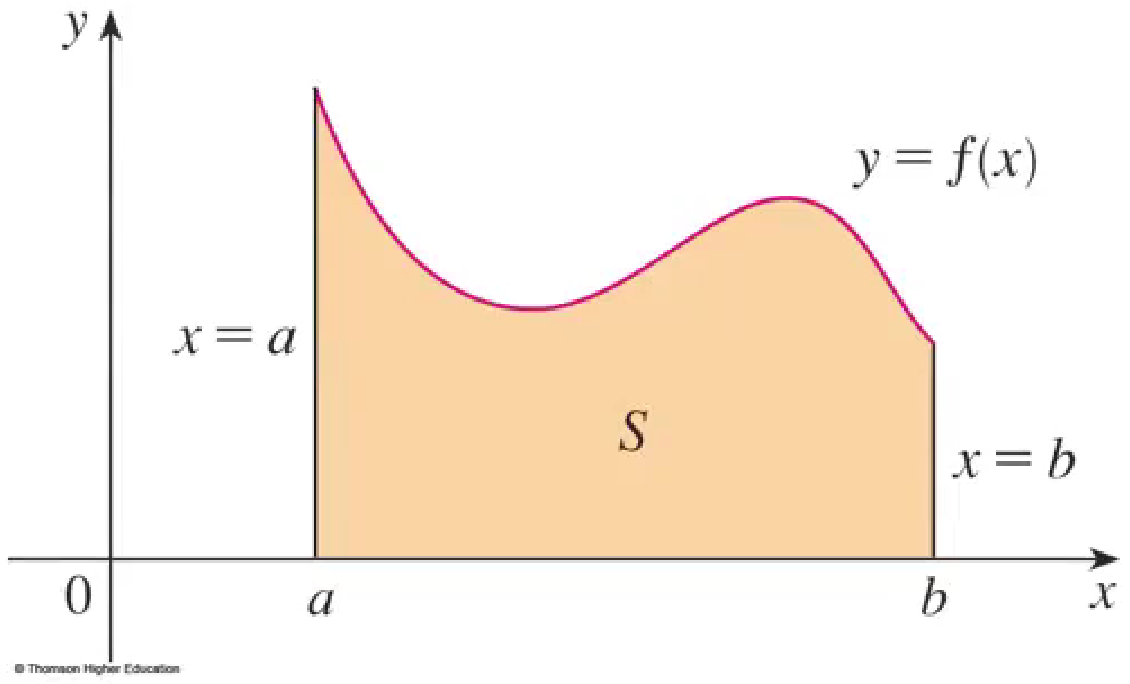
\includegraphics[scale=0.5]{images/area}
        \centering
    \end{figure}

    \noindent\enclose{
        \textbf{DEFINE.}
        We begin by attempting to solve the area problem. 
        Find the area of the region \textit{S} that lies under the curve \inline{y = f (x)} from \textit{a} to \textit{b}.
        This means that \textit{S}, illustrated here, is bounded by:
        \begin{itemize}
            \item[-] The graph of a continuous function \textit{f} where \inline{f (x) \leq{} 0}.
            \item[-] The vertical lines \inline{x = a} and \inline{x = b}. 
            \item[-] The \textit{x}-axis.
        \end{itemize}

        \textbf{NOTE.}
        The goal is to use \hl{limit} in trying to find the area under a curve.
        However, it isn't so easy to find the area of a region with curved sides.
        Hence, a part of the area problem is to make this intuitive idea precise by giving an \hl{exact definition of area}.

        \bigskip\textbf{PLAN.}
        We first approximate the region \textit{S} by rectangles and then we take the \hl{limit of the sum and the areas of these rectangles} as we increase the number of rectangles.
    }

    \newpage\textbf{EXAMPLE 5.1.0.}
    
    \begin{figure}[h]
        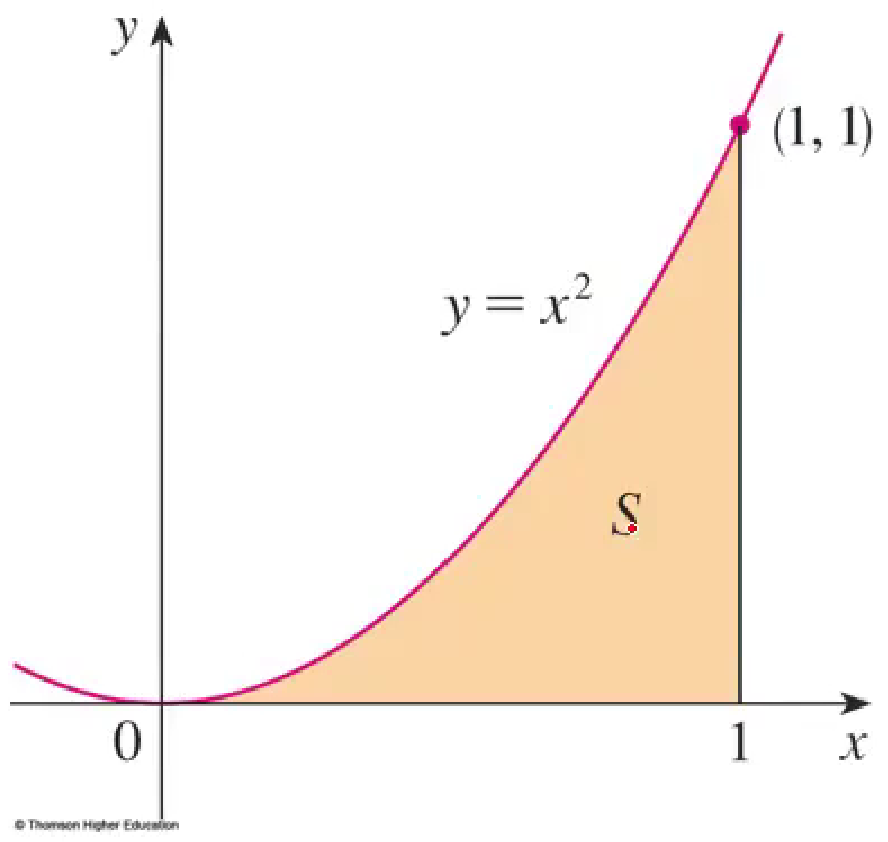
\includegraphics[scale=0.5]{images/area01}
        \centering
    \end{figure}

    \begin{itemize}
        \item[-] 
        Use rectangles to estimate the area under the parabola \inline{y = x^2} from 0 to 1, the parabolic region \textit{S} illustrated above.
        We first notice that the area of \textit{S} must be somewhere between 0 and 1, because \textit{S} is contained in a square with side length 1.
        Do suppose we divide \textit{S} into four strips: \inline{S_1}, \inline{S_2}, \inline{S_3}, and \inline{S_4} by drawing the vertical lines \textit{x} = 1/4, \textit{x} = 1/2, \textit{x} = 3/4.
        \item[-] 
        The heights of these rectangles are the values of the function \inline{f (x) = x^2} at the right endpoints of the subintervals [0, 1/4], [1/4, 1/2], [1/2, 3/4], and [3/4, 1].
        Hence, if we let \inline{R_4} be the sum of the areas of these approximating rectangles, we get:
        \proving{
            R_4 &= \frac{1}{4} \point{} {\left(\frac{1}{4}\right)}^2 + \frac{1}{4} \point{} {\left(\frac{1}{2}\right)}^2 + \frac{1}{4} \point{} {\left(\frac{3}{4}\right)}^2 + \frac{1}{4} \point{} 1^2 \\
            &= \frac{15}{32} \\
            &= 0.46875
        }
        \inline{\therefore{}} The area \textit{A} of \textit{S} is less than \inline{R_4}; so, \textit{A} \textless{} 0.46875.
        \item[-]
        We could use the smaller rectangles by taking the height as values of \textit{f} at the left endpoints of the subintervals.
        Hence, the sum of the areas of these approximating rectangles is:
        \proving{
            L_4 &= \frac{1}{4} \point{} {0}^2 + \frac{1}{4} \point{} {\left(\frac{1}{4}\right)}^2 + \frac{1}{4} \point{} {\left(\frac{1}{2}\right)}^2 + \frac{1}{4} \point{} {\left(\frac{3}{4}\right)}^2 \\
            &= \frac{7}{32} \\
            &= 0.21875
        }
        \inline{\therefore{}} We conclude that the lower and upper estimates of \textit{A}: \inline{0.21875 < A < 0.46875}.
        \item[-] As we increase the number of rectangles, denoted as \textit{n}, \textit{R} and \textit{L} approaches a certain value; in this case, 1/3.
    \end{itemize}

    \newpage\follow\enclose{
        \textbf{DEFINE.}
        Hence, we define the exact area to be \hl{the limit of the sums of the areas of the approximating rectangles}, that is, \block{A = \lim_{n \rightarrow{} \infty{}} R_n = \lim_{n \rightarrow{} \infty{}} L_n = \frac{1}{3}}
    }

    \follow\enclose{
        \textbf{DEFINE.}
        The area \textit{A} of the region \textit{S} that lies under the graph of the continuous function \textit{f} is the limit of the \hl{sum of the areas of approximating rectangles} such that \block{A = \lim_{n \rightarrow{} \infty{}} R_n = \lim_{n \rightarrow{} \infty{}} \left[f (x_1) \triangle{x} + f (x_2) \triangle{x} + \ldots{} + f (x_n) \triangle{x}\right] = \lim_{n \rightarrow{} \infty{}} \sum_{i = 1}^n f (x_i^*) \triangle{x}}
    }

    \follow\enclose{       
        \textbf{DEFINE.}
        In the mathematical notation, \block{\int_{a}^{b} f (x) \, dx} where
        \begin{conditions}
            f (x) & Integrand \\
            a & Lower Limit \\
            b & Upper Limit
        \end{conditions}
        \textbf{NOTE.}
        The symbol \inline{\int{}} was introduced by Leibniz and is called an integral sign.
    }

    \follow\textbf{EXAMPLE 5.1.1.}
    Through interpreting it as the measure of the area of a plane region, compute the value of the intergral:
    \proving{
        \int_{0}^{3} x \, dx &= \frac{1}{2} (3) (3)     & Area &= \frac{1}{2} \, bh \\
        &= \frac{9}{2}
    }

    \follow\textbf{EXAMPLE 5.1.2.}
    Compute the value of the integral:
    \proving{
        \int_{-3}^{3} \sqrt{9 -x^2} \, dx &= \frac{1}{2} \pi{} {(3)}^2  & Area &= \frac{1}{2} \pi{} r^2 \\
        &= \frac{9 \pi{}}{2}
    }

\newpage\section{The Fundamental Theorem of the Calculus}

    
    \enclose{
        \textbf{DEFINE.}
        The first fundamental theorem of calculus ties the idea of \hl{derivative} and the concept of \hl{definite integral}.
        This theorem defines the derivative of a function that is a definite integral having a variable upper limit.
    }

    \subsection{The First Fundamental Theorem of Calculus}

        \enclose{
            \textbf{DEFINE.}
            Let \textit{f} be a continuous on the closed interval \inline{[a, b]} and let \textit{x} be a number in \inline{[a, b]}.
            If \textit{g} is the function defined by \block{g (x) = \int_{a}^{x} f (t) \, dt} then \block{g ' (x) = f (x)} or equivalently, \block{\frac{d}{dx} \int_{a}^{x} f (t) \, dt = f (x)}.
        }

        \follow\textbf{EXAMPLE 6.1.1.}
        Compute the following derivative \inline{\frac{d}{dx} \int_{\pi{}}^{x} \cot^2{t} \, dt}.
        \proving{
            &= \cot^2{x}
        }

        \follow\textbf{EXAMPLE 6.1.2.}
        Compute the following derivative \inline{\frac{d}{dx} \int_{\pi{}}^{x^2} \cot^2{t} \, dt}.
        \proving{
            &= g' (x^2) \, \frac{d}{dx} \, (x^2)    & g (x) &= \int_{\pi{}}^{x} \cot^2{t} \, dt \\
            &= \cot^2{(x^2)} \point{} 2x            & g' (x) &= \cot^2{x} \\
            &= 2x \cot^2{(x^2)}
        }

        \follow\textbf{EXAMPLE 6.1.3.}
        Compute the following derivative \inline{\frac{d}{dx} \int_{1}^{\sqrt{x}} \frac{s^2}{s^2 + 1} \, ds}.
        \proving{
            &= \frac{{(\sqrt{x})}^2}{{(\sqrt{x})}^2 + 1} \point{} \frac{d}{dx} (\sqrt{x})   & \frac{d}{dx} (x^{1/2}) &= \frac{1}{2} x^{-1/2} \\
            &= \frac{x}{x + 1} \point{} \frac{1}{2\sqrt{x}}                                 & &= \frac{1}{2\sqrt{x}}
        }

        \newpage\follow\textbf{EXAMPLE 6.1.4.}
        Compute the following derivative \inline{\frac{d}{dx} \int_{x}^{2} \left[\cos{} (t^2) + t \right] \, dt}.
        \proving{
            &= \frac{d}{dx} \Big[-\int_{2}^{x} [\cos{} (t^2) + t] \, dt\Big] \\
            &= -\frac{d}{dx} \int_{2}^{x} [\cos{} (t^2) + t] \, dt \\
            &= -[\cos{} (x^2) + x]
        }

        \follow\textbf{EXAMPLE 6.1.5.}
        Compute the following derivative \inline{\frac{d}{dx} \int_{\tan{x}}^{x^2} \frac{1}{\sqrt{2 + t^4}} \, dt}.

\end{document}